% ============================================================
% 3  The lattice model, its order parameter, true LRO
% Frames 1 and 2 share ONE layout: row 1 (cartoon + operator), row 2 (figure 0.58 | verdicts 0.40)
% ============================================================
\begin{frame}[t]
\ft{First try: a single spin flip}\par
\vspace{0.2cm}
\begin{columns}[c]
\begin{column}{0.30\textwidth}
\centering
\begin{tikzpicture}[every pic/.style={scale=0.6}]
 \draw[gray,thick] (-0.2,0)--(1.25,0); \foreach \x in {0,0.35,0.7,1.05} \fill[gray] (\x,0) circle (0.04);
 \path (0.35,0.25) pic {edn};
 \draw[-{Stealth[length=4pt]},thick] (1.4,0.25)--(1.75,0.25);
 \begin{scope}[xshift=1.95cm]
 \draw[gray,thick] (-0.2,0)--(1.25,0); \foreach \x in {0,0.35,0.7,1.05} \fill[gray] (\x,0) circle (0.04);
 \path (0.35,0.25) pic {eup};
 \end{scope}
\end{tikzpicture}\par
{\footnotesize one spin flip\par}
\end{column}
\begin{column}{0.68\textwidth}
\setlength{\fboxsep}{2pt}\centering
\parbox[c][1.7cm][c]{\linewidth}{\centering
{\small$S^+_i\sim\underbrace{\colorbox{citron!40}{$\mystrut e^{-i\sqrt{2\pi}\theta_s}$}}_{\text{\scriptsize$\theta$: good}}\Big[\cos\sqrt{2\pi}\phi_s+\alt<2->{\underbrace{\colorbox{pumpkin!40}{$\mystrut\cos(\sqrt{2\pi}\phi_c+2k_Fx)$}}_{\text{\scriptsize charge Luttinger liquid}}}{\underbrace{\colorbox{white}{$\mystrut\cos(\sqrt{2\pi}\phi_c+2k_Fx)$}}_{\text{\scriptsize\phantom{charge Luttinger liquid}}}}\Big]$\par}}
\end{column}
\end{columns}
\vspace{0.3cm}
\onslide<2->{%
\begin{columns}[T]
\begin{column}{0.58\textwidth}
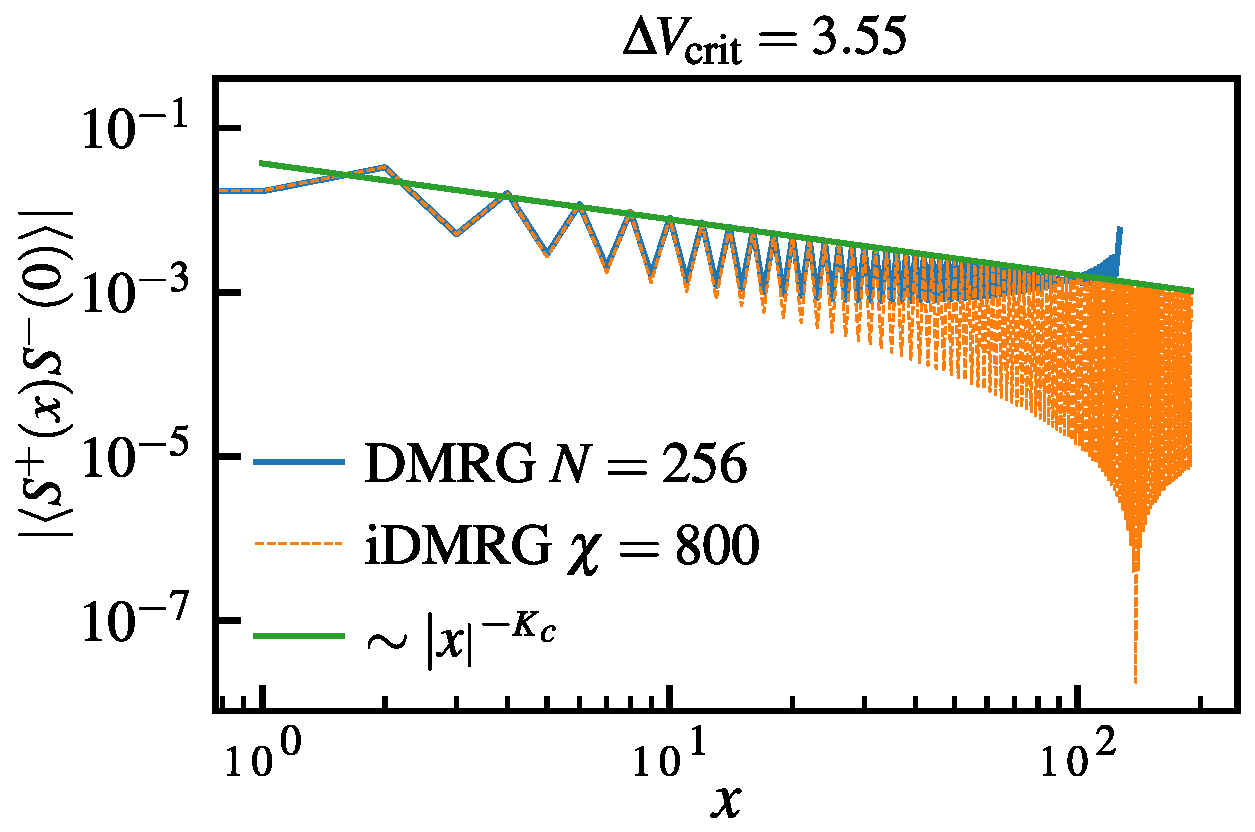
\includegraphics[width=\linewidth]{figures/paper_fig2_splus.png}\par
\vspace{0.05cm}
{\tiny\color{citegray} Andriyakhina, Shankar, Senthil, Shi, arXiv:2609.38581 (2026)\par}
\end{column}
\begin{column}{0.40\textwidth}
\raggedright
\textbf{\color{cQCP}critical point}\\[3pt]
$\langle S^+_xS^-_0\rangle$: still a power law\\[3pt]
{\scriptsize the charge part never orders\par}
\end{column}
\end{columns}}
\end{frame}
% Notes: Step 1: S^+ flips one spin, rotating the in-plane spin, and contains the theta vertex, so it is the natural candidate.
% Notes: Step 2: But in an itinerant chain it also drags the charge sector along (the 2k_F part). The charge Luttinger liquid stays critical, so even at the critical point S^+ only has a power law (Fig. 2).


\begin{frame}[t]
\ft{Pair the flips: true long-range order}\par
\vspace{0.2cm}
\begin{columns}[c]
\begin{column}{0.30\textwidth}
\centering
\begin{tikzpicture}[every pic/.style={scale=0.6}]
 \draw[gray,thick] (-0.2,0)--(1.25,0); \foreach \x in {0,0.35,0.7,1.05} \fill[gray] (\x,0) circle (0.04);
 \path (0.35,0.25) pic {edn}; \path (0.7,0.25) pic {edn};
 \draw[-{Stealth[length=4pt]},thick] (1.4,0.25)--(1.75,0.25);
 \begin{scope}[xshift=1.95cm]
 \draw[gray,thick] (-0.2,0)--(1.25,0); \foreach \x in {0,0.35,0.7,1.05} \fill[gray] (\x,0) circle (0.04);
 \path (0.35,0.25) pic {eup}; \path (0.7,0.25) pic {eup};
 \end{scope}
\end{tikzpicture}\par
{\footnotesize two spin flips\par}
\end{column}
\begin{column}{0.68\textwidth}
\setlength{\fboxsep}{2pt}\centering
\parbox[c][1.7cm][c]{\linewidth}{\centering
{\small$\mathcal O_i=S^+_iS^+_{i+1}\sim\underbrace{\colorbox{citron!40}{$\mystrut e^{-i\sqrt{8\pi}\theta_s}=e^{-2i\theta}$}}_{\text{\scriptsize only $\theta$: charge cancels}}$\par}
\vspace{0.1cm}
{\scriptsize spin 2: a spin nematic\par}}
\end{column}
\end{columns}
\vspace{0.3cm}
\onslide<2->{%
\begin{columns}[T]
\begin{column}{0.58\textwidth}
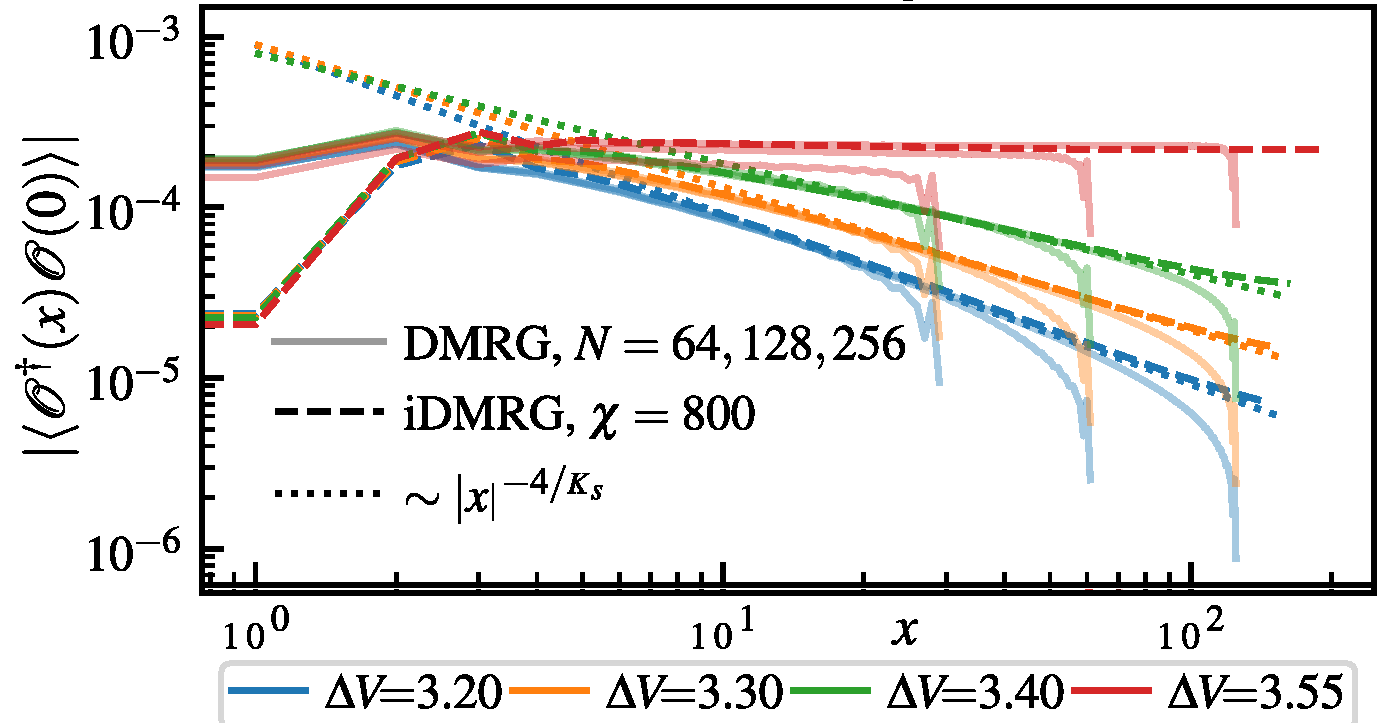
\includegraphics[width=\linewidth]{figures/paper_fig1_nematic.png}\par
\vspace{0.05cm}
{\tiny\color{citegray} Andriyakhina, Shankar, Senthil, Shi, arXiv:2609.38581 (2026)\par}
\end{column}
\begin{column}{0.40\textwidth}
\raggedright
\textbf{\color{cLL}Luttinger liquid}\\[3pt]
$\langle\mathcal O^\dagger_x\mathcal O_0\rangle\sim|x|^{-4/K_s}$\\[3pt]
{\scriptsize slower as $K_s$ grows\par}
\vspace{0.3cm}
\onslide<3->{\textbf{\color{cQCP}critical point}\\[3pt]
$\langle\mathcal O^\dagger_x\mathcal O_0\rangle\to$ const\\[3pt]
{\scriptsize $\langle S^z\rangle=\langle S^\pm\rangle=0$: nematic order only\par}}
\end{column}
\end{columns}}
\onslide<3->{\tk{An ordered critical point in one dimension}}
\end{frame}
% Notes: Step 1: Flip two neighbours: the charge parts cancel (Klein factors, supplement). A pure theta vertex, e^{-2 i theta}, spin 2: a spin-nematic order parameter.
% Notes: Step 2: Nematic correlator vs distance, log-log. Blue/orange/green: Luttinger liquid at increasing Delta V; dotted lines are |x|^{-4/K_s} with K_s from the LL fits: the decay gets slower as we approach the QCP.
% Notes: Step 3: red, at Delta V_crit: the correlator saturates to a constant, both in finite chains (faded, up to boundary effects) and in iDMRG (dashed). True long-range order. No magnetization, no ordinary transverse order (S+S- is only QLRO), but spin-nematic LRO. The naive "K_s -> infinity" picture gives the right answer here, but the critical point is not a Luttinger liquid: next slides.
